%!TEX root = ../dokumentation.tex
\section{Testfälle erfassen}
Die Testfälle beziehen sich auf die Ausführbarkeit der MUSS- und KANN-Ziele.
Einige Ziele sind jeweils im Admin und in der Wochenansicht ausführbar.
Ziele die auch in der Wochenansicht vorhanden sind, werde ich nicht im Admin testen, da es dieselben Prozesse sind.
\begin{table}[!ht]
\begin{center}
    \begin{tabular}{llp{12cm}l}
        \toprule Nr & Ziel-Funktion & Testfrage \\
        \midrule 1 & 1 & Kann der Benutzer eine neue Task erfassen?\\
        \midrule 2 & 2 & Kann der Benutzer einer Task einen Namen geben? \\
        \midrule 3 & 3 & Kann der Benutzer einer Task ein Datum geben? \\
        \midrule 4 & 4 & Kann der Benutzer einer Task eine Person zuweisen? \\
        \midrule 5 & 5 & Kann der Benutzer einer Task eine Dauer geben? \\
        \midrule 6 & 6 & Kann der Benutzer eine Task bearbeiten? \\ 
        \midrule 7 & 7 & Kann der Benutzer eine Task löschen? \\
        \midrule 8 & 8 & Kann der Benutzer einer Person einen Sperrtag zuweisen? \\
        \midrule 9 & 9 & Kann der Benutzer einem Sperrtag einen Namen geben? \\
        \midrule 10 & 10 & Kann der Benutzer einen Sperrtag bearbeiten?\\
        \midrule 11 & 11 & Kann der Benutzer einen Sperrtag löschen?\\
        \midrule 12 & 12 & Kann der Benutzer eine Task einem Projekt zuweisen?\\
        \midrule 13 & 13 & Kann der Benutzer eine Person zum Wochenplaner hinzufügen?\\
        \midrule 14 & 14 & Kann der Benutzer eine Person als Partner kennzeichnen?\\
        \midrule 15 & 15 & Kann der Benutzer eine Task duplizieren?\\
        \midrule 16 & 16 & Kann der Benutzer einem Sperrtag ein Start- \& Enddatum geben?\\
        \midrule 17 & 17 & Erscheint eine Warnmeldung wenn Taskdauer grösser als 8h \\
        \midrule 18 & 18 & Kann der Benutzer Tasks in einem Tag sortieren?\\
        \bottomrule
    \end{tabular}
    \caption{Zu erfüllende Funktionen des Prototypen}
    \label{tab:testing_muss_funktionen}
\end{center}
\end{table}
\section{Testmethoden}
GUI Unit-Tests zu machen hätten den Rahmen meiner Arbeit gesprengt.
Mit Selenium kann man Websiten automatisiert getestet werden. Alle Interaktion die ein User machen kann, könnten so getestet werden.
Dies ist aber nur für grössere Webapplikationen sinnvoll.\\
Deshalb teste ich die User-Interaktionen manuell und prüfe über die Konsole was ich für eine Antwort erhalten habe. Dazu wird natürlich noch ein visuelles Feedback über HTML ausgegeben.
Ich werde die definierten Testfälle durchführen und mit Screenshots dokumentieren ob wie sie ausgeführt werden.
Auf den Bildern ist ausserdem (sofern vorhanden) der REST-Call aufgelistet, der die Kommunikation mit dem Server darstellt.
\clearpage
\begin{figure}[htbp]
    \centering
        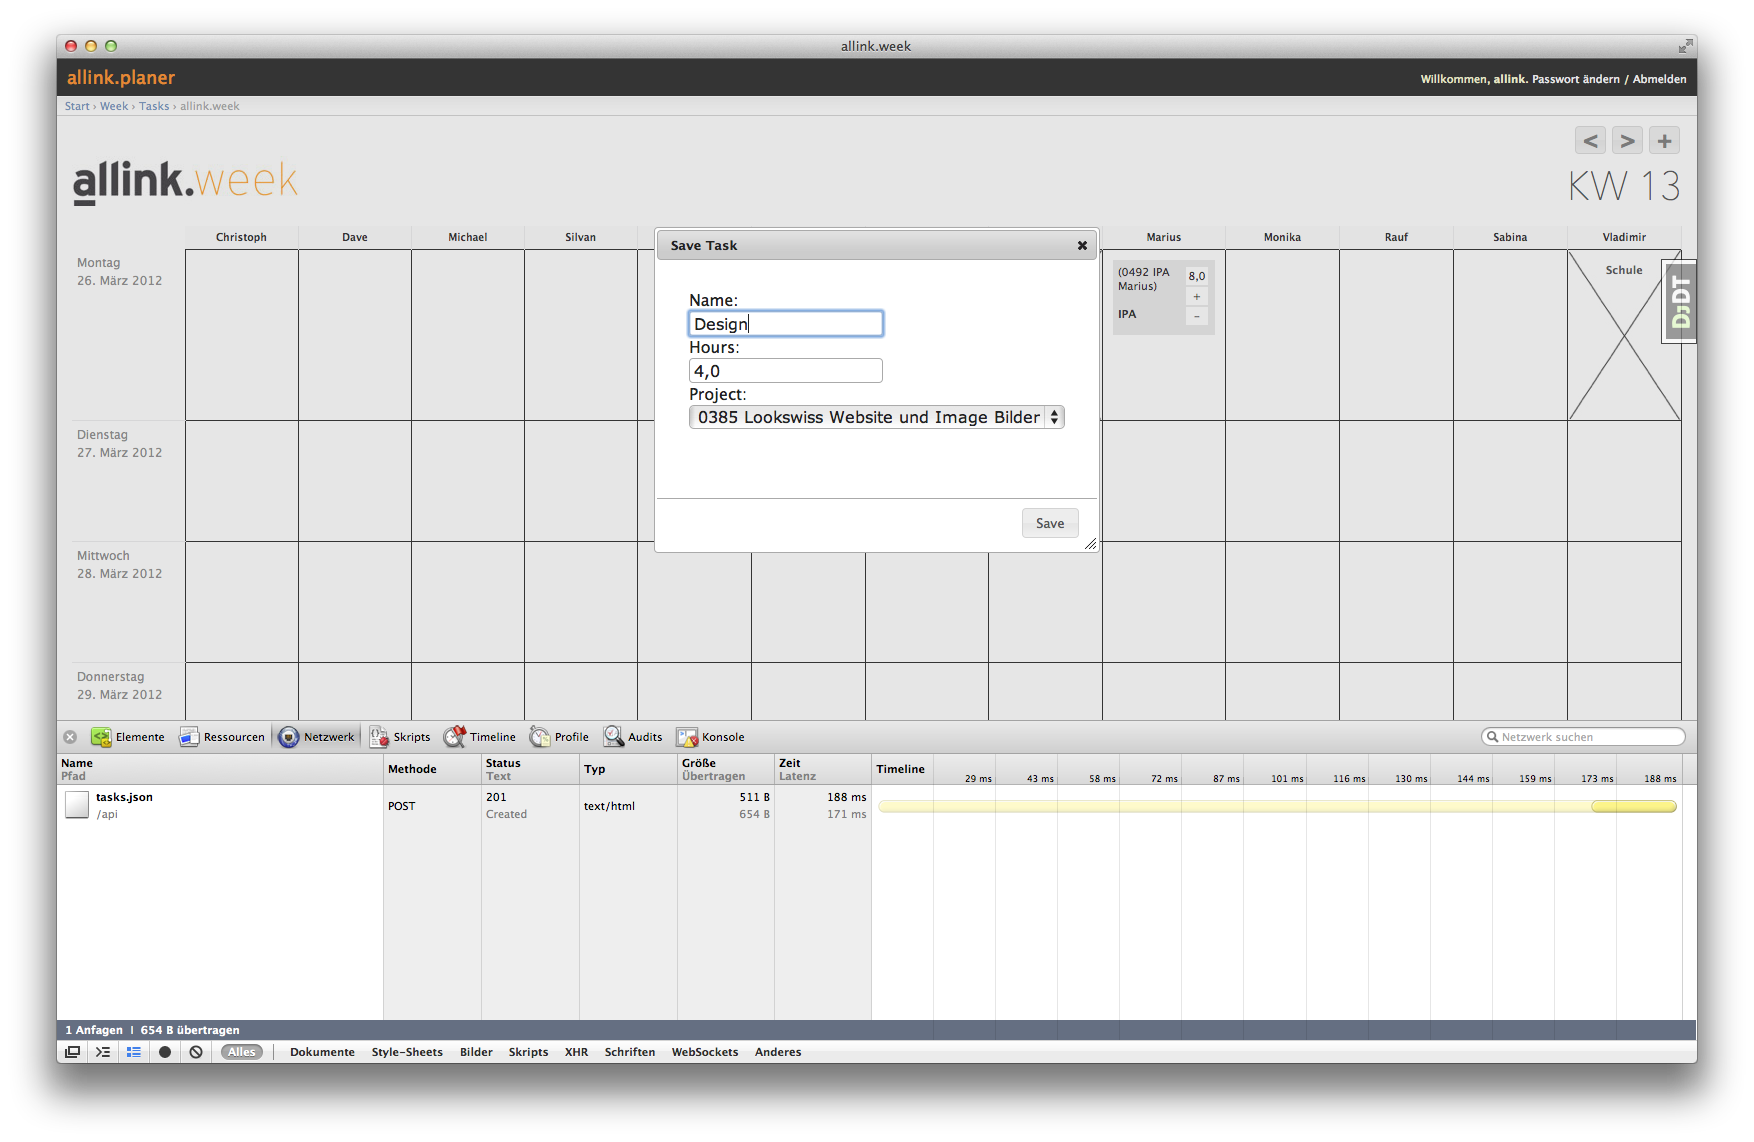
\includegraphics[height=0.85\textwidth,angle=90]{bilder/testing/Task_erstellen.png}
    \caption{Abgedeckte Ziele: Nr. 1, 2, 3, 4, 5, 12}
    \label{fig:bilder_testing_Task erstellen}
\end{figure}
\begin{figure}[htbp]
    \centering
        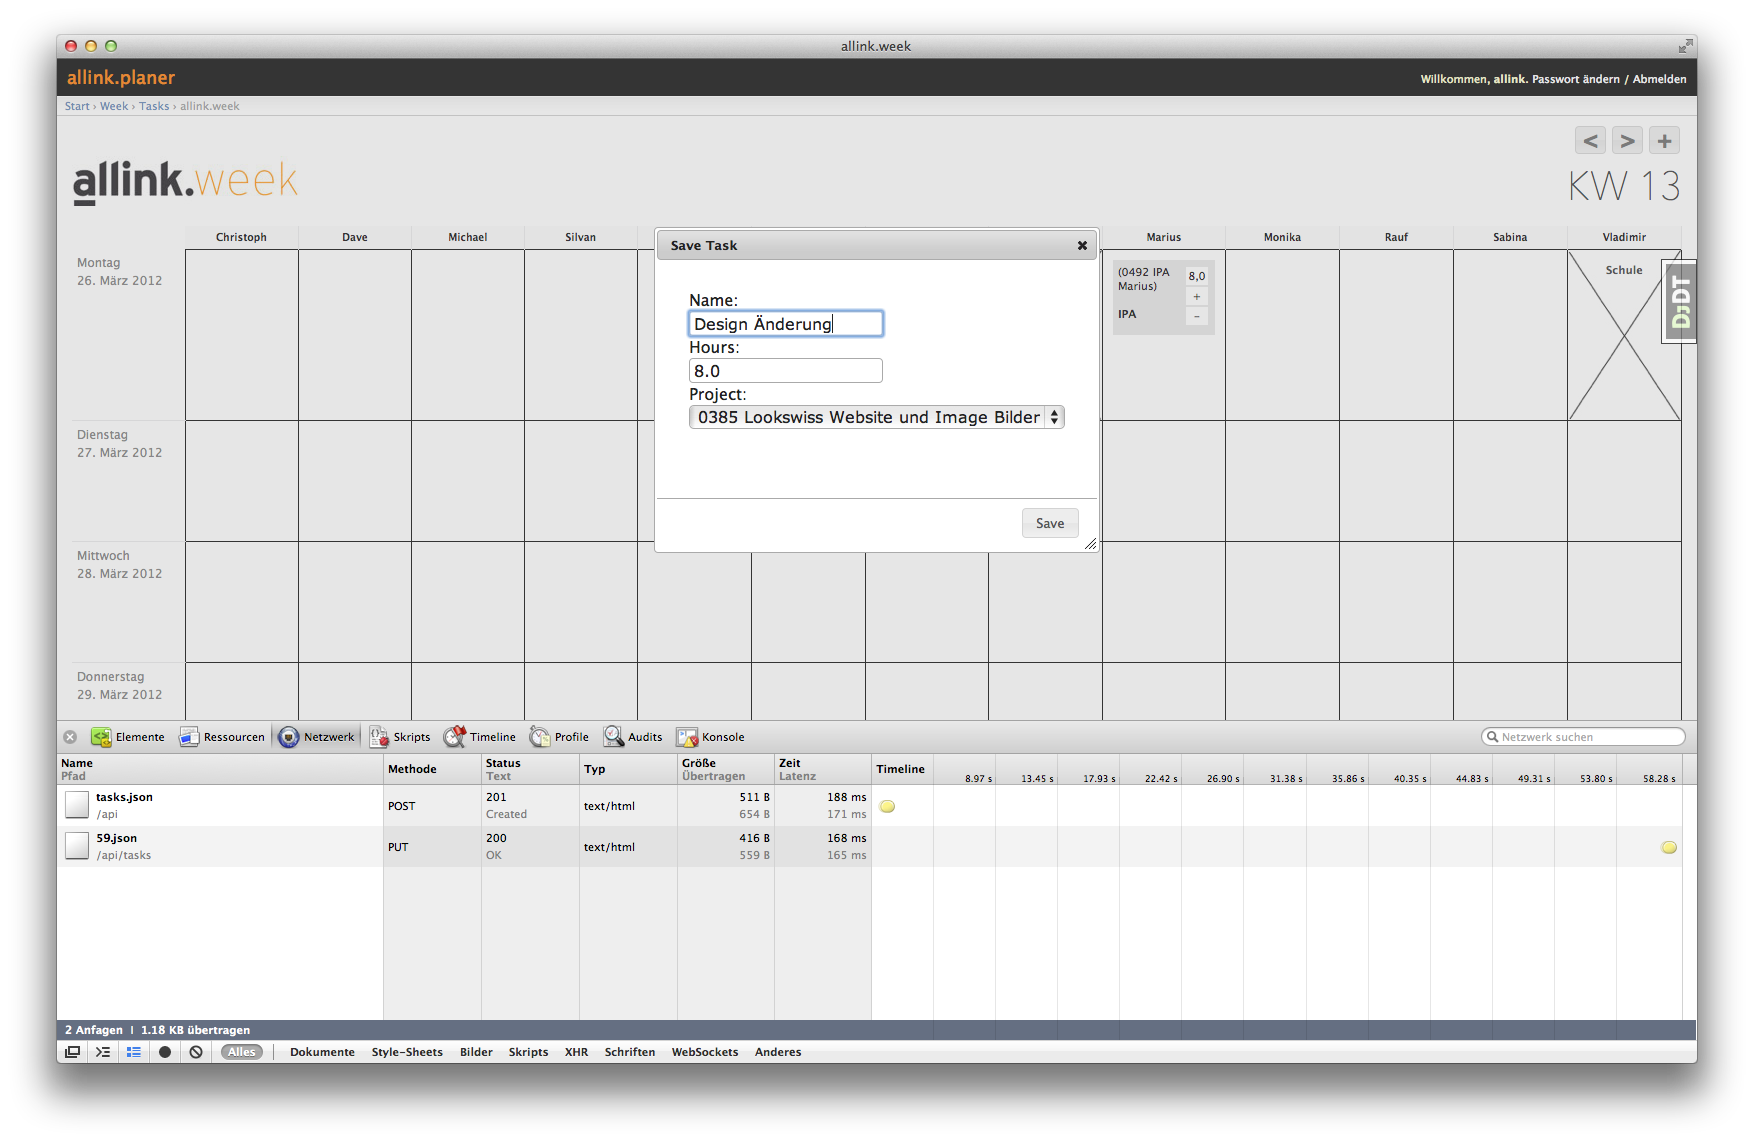
\includegraphics[height=0.85\textwidth,angle=90]{bilder/testing/Task_bearbeiten.png}
    \caption{Abgedeckte Ziele: Nr. 6}
    \label{fig:bilder_testing_Task_bearbeiten}
\end{figure}
\begin{figure}[htbp]
    \centering
        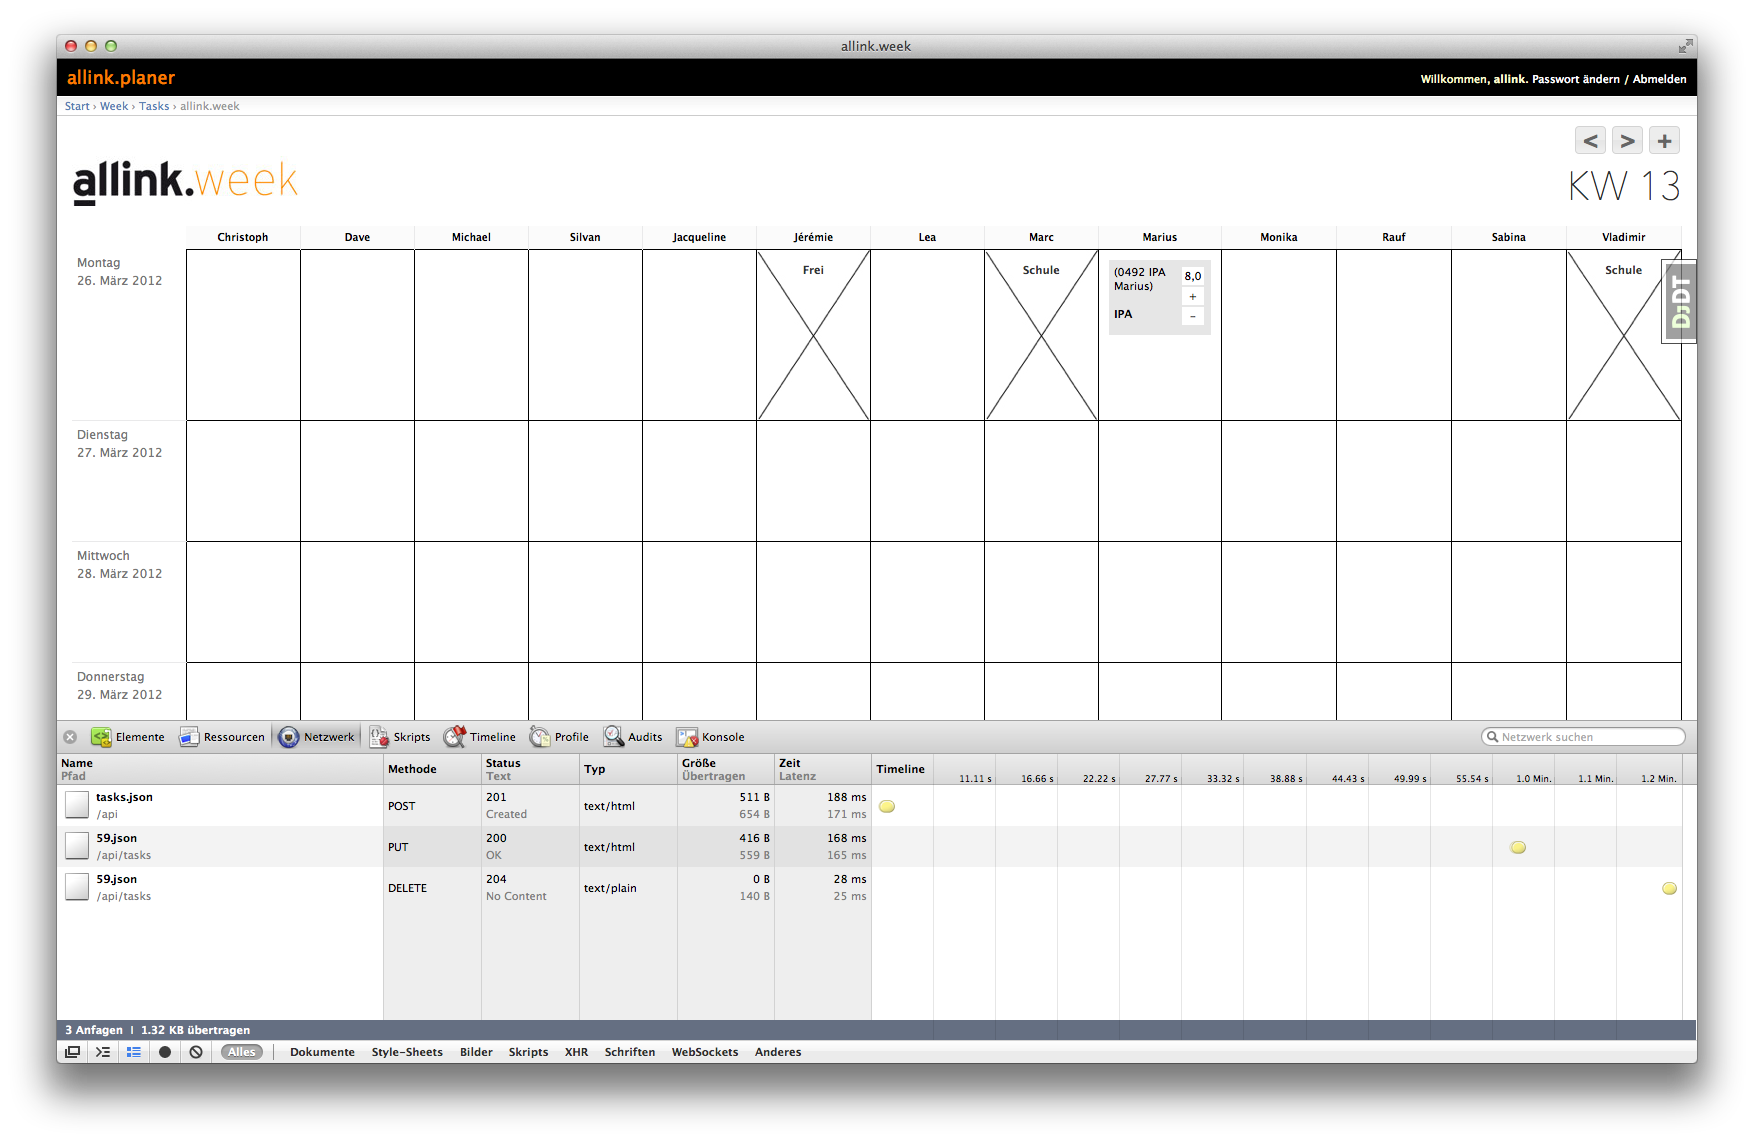
\includegraphics[height=0.85\textwidth,angle=90]{bilder/testing/Task_loeschen.png}
    \caption{Abgedeckte Ziele: Nr. 7}
    \label{fig:bilder_testing_Task_loeschen}
\end{figure}
\begin{figure}[htbp]
    \centering
        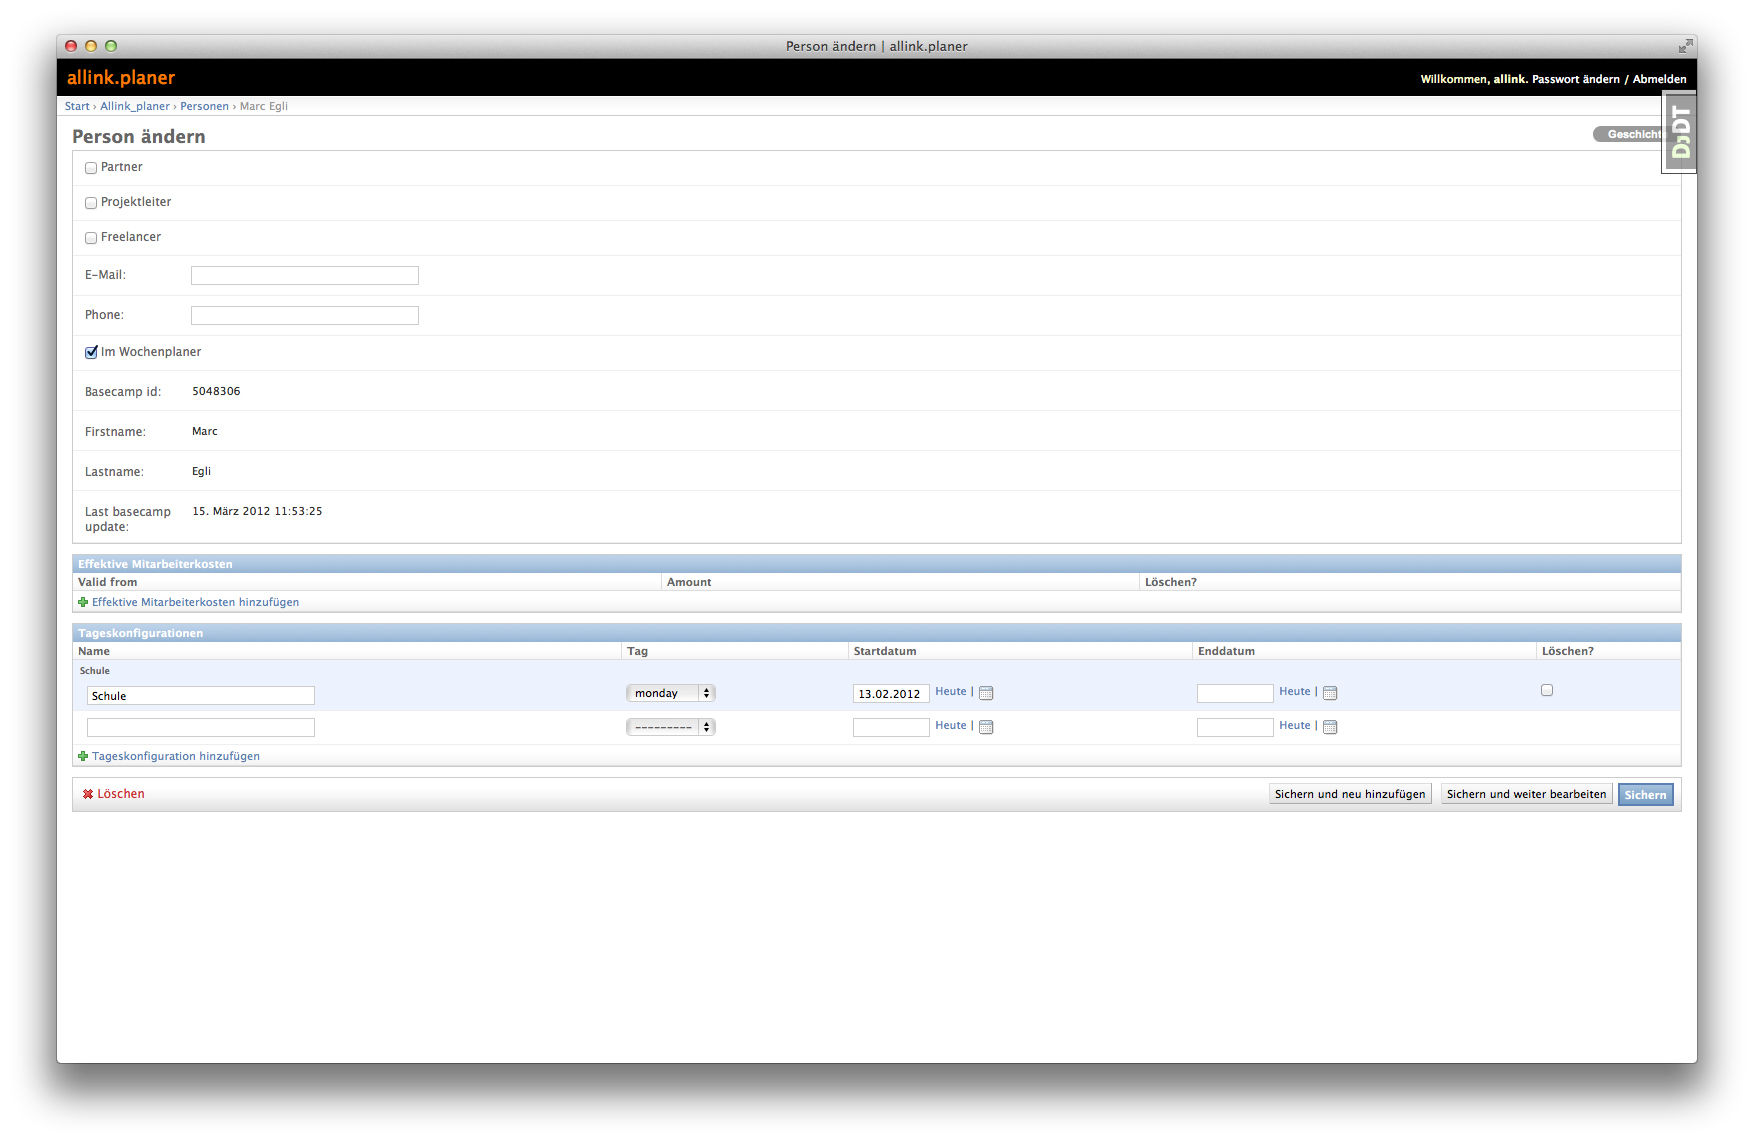
\includegraphics[height=0.85\textwidth,angle=90]{bilder/testing/Sperrtag_erstellen.png}
    \caption{Abgedeckte Ziele: Nr. 8, 9}
    \label{fig:bilder_testing_Sperrtag_erstellen}
\end{figure}
\begin{figure}[htbp]
    \centering
        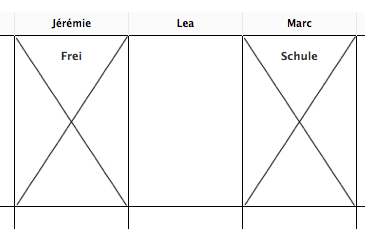
\includegraphics[height=0.85\textwidth,angle=90]{bilder/testing/Sperrtag_Person_zuweisen.png}
    \caption{Abgedeckte Ziele: Nr. 8, 9}
    \label{fig:bilder_testing_Sperrtag_Person_zuweisen}
\end{figure}
\begin{figure}[htbp]
    \centering
        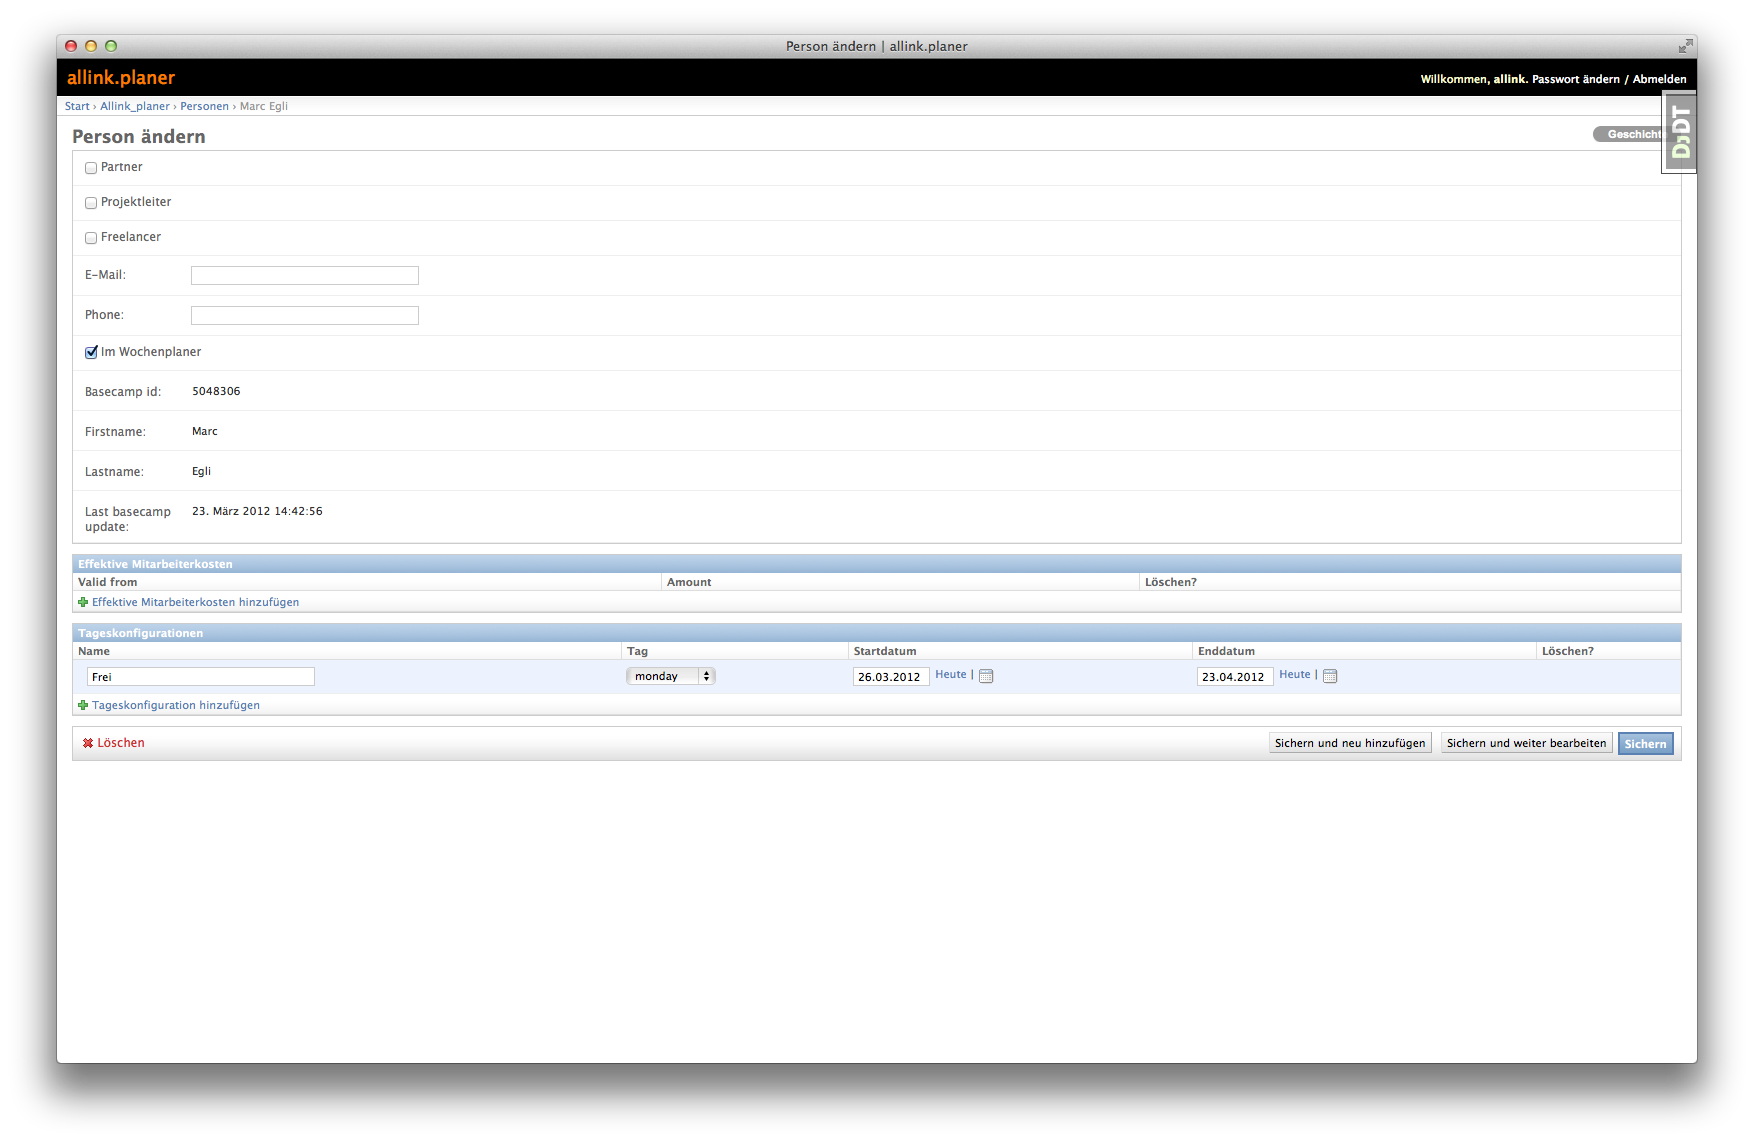
\includegraphics[height=0.85\textwidth,angle=90]{bilder/testing/Sperrtag_bearbeiten.png}
    \caption{Abgedeckte Ziele: Nr. 10}
    \label{fig:bilder_testing_Sperrtag_bearbeiten}
\end{figure}
\begin{figure}[htbp]
    \centering
        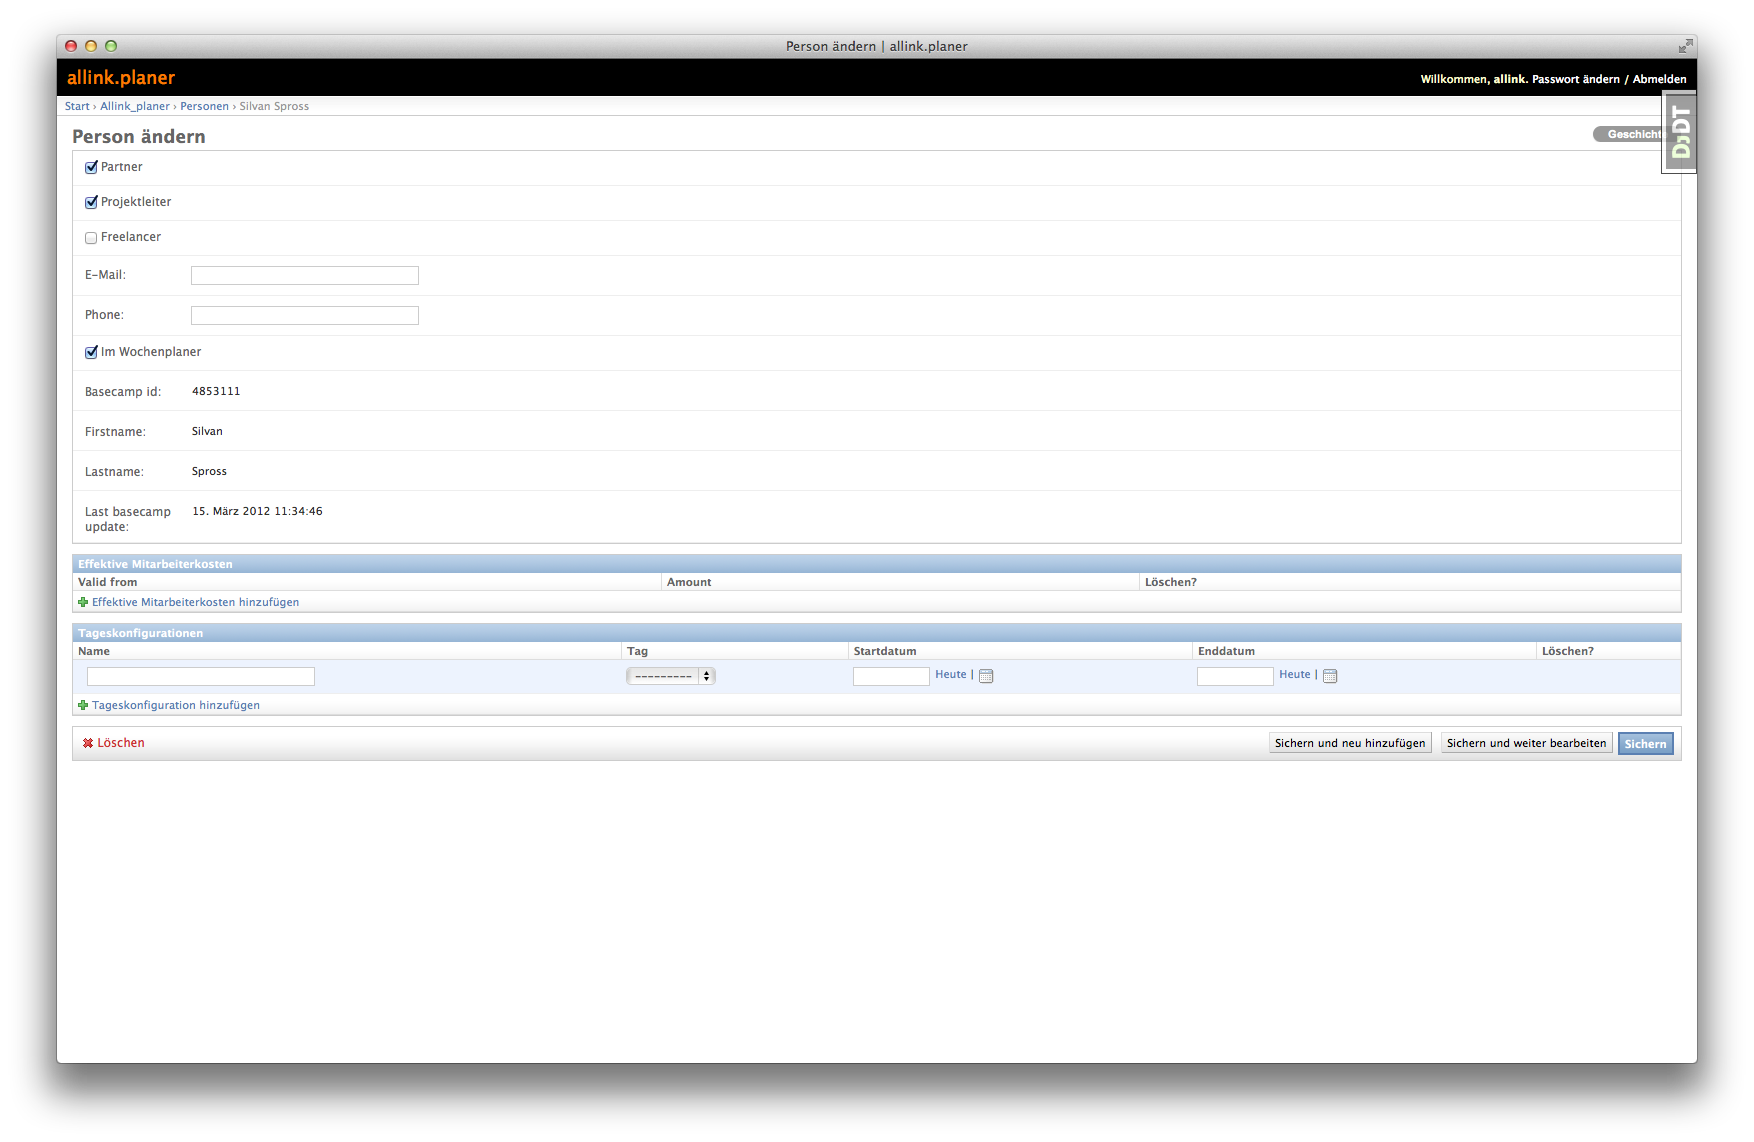
\includegraphics[height=0.85\textwidth,angle=90]{bilder/testing/Sperrtag_loeschen.png}
    \caption{Abgedeckte Ziele: Nr. 11}
    \label{fig:bilder_testing_Sperrtag_loeschen}
\end{figure}
\begin{figure}[htbp]
    \centering
        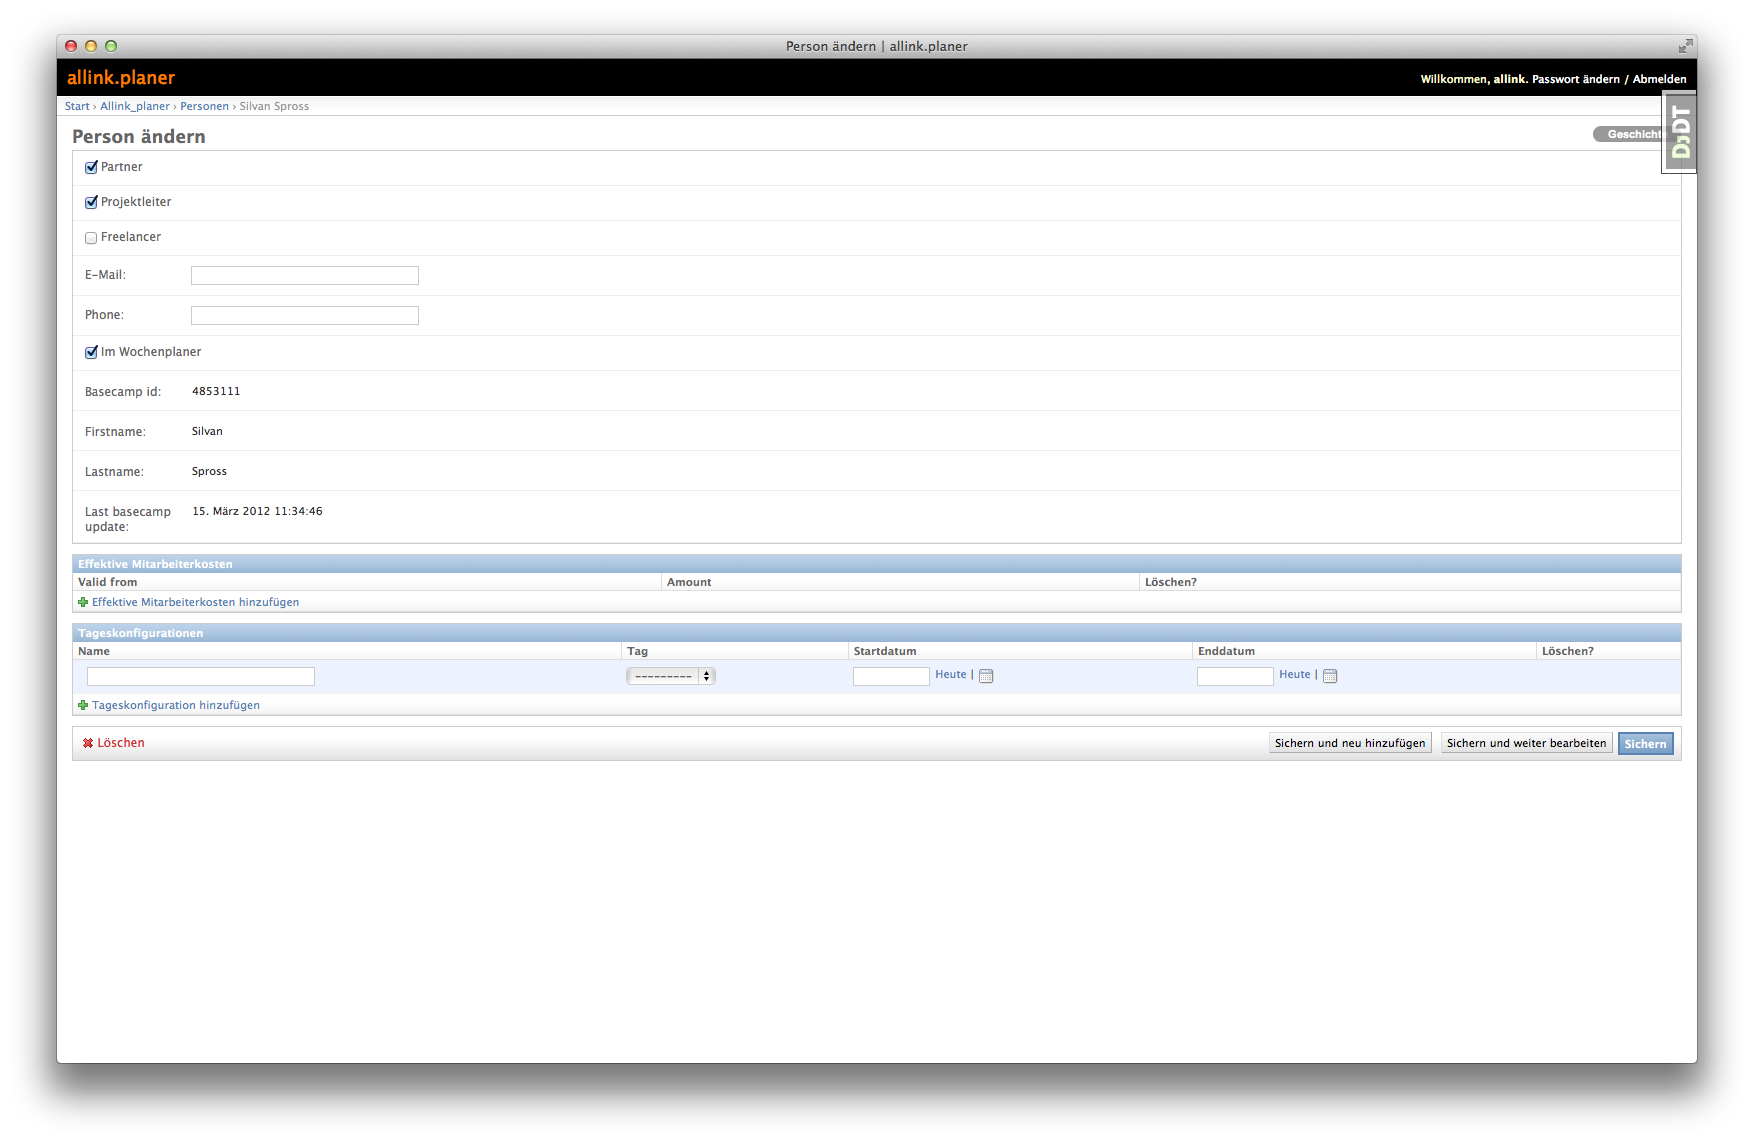
\includegraphics[height=0.85\textwidth,angle=90]{bilder/testing/Person_wochenplaner_partner.png}
    \caption{Abgedeckte Ziele: Nr. 13, 14}
    \label{fig:bilder_testing_Person_wochenplaner_partner}
\end{figure}
\begin{figure}[htbp]
    \centering
        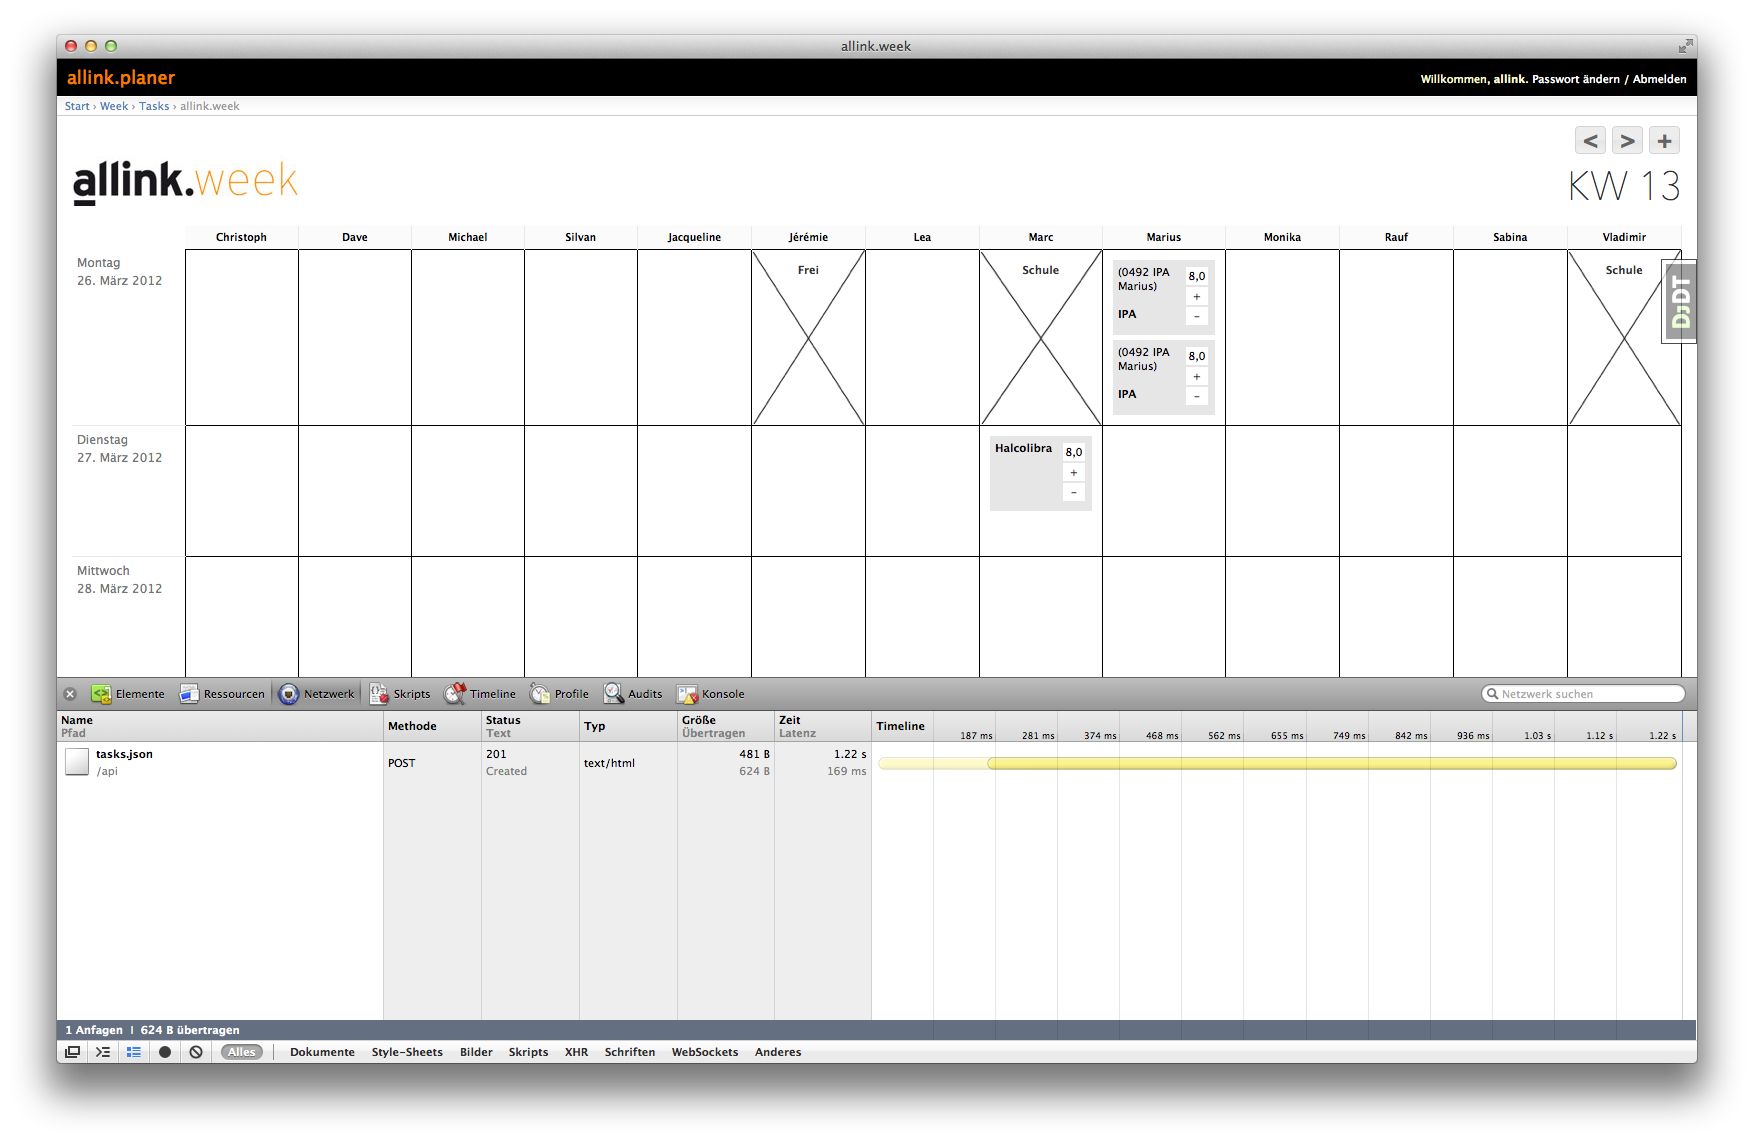
\includegraphics[height=0.85\textwidth,angle=90]{bilder/testing/Task_duplizieren.png}
    \caption{Abgedeckte Ziele: Nr. 15}
    \label{fig:bilder_testing_Task_duplizieren}
\end{figure}
\begin{figure}[htbp]
    \centering
        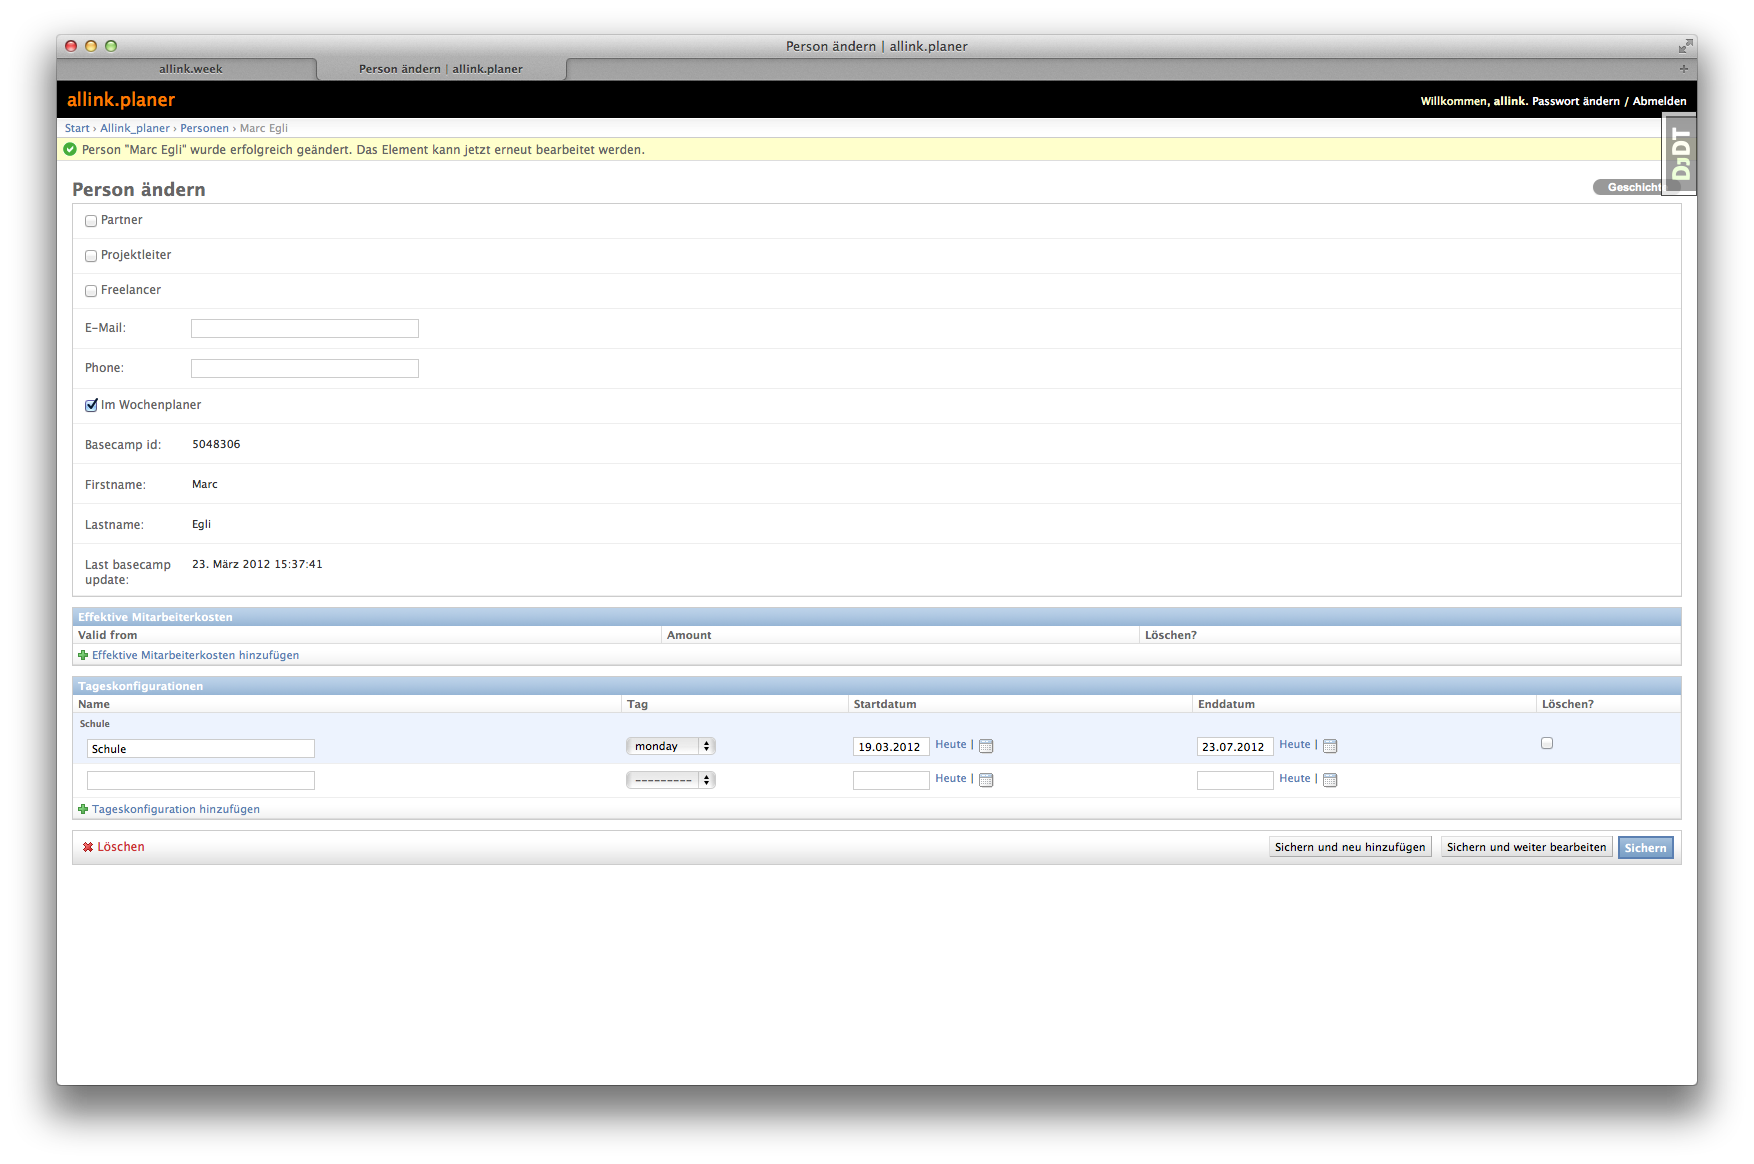
\includegraphics[height=0.85\textwidth,angle=90]{bilder/testing/Sperrtag_start_end.png}
    \caption{Abgedeckte Ziele: Nr. 16}
    \label{fig:bilder_testing_Sperrtag_start_end}
\end{figure}
\begin{figure}[htbp]
    \centering
        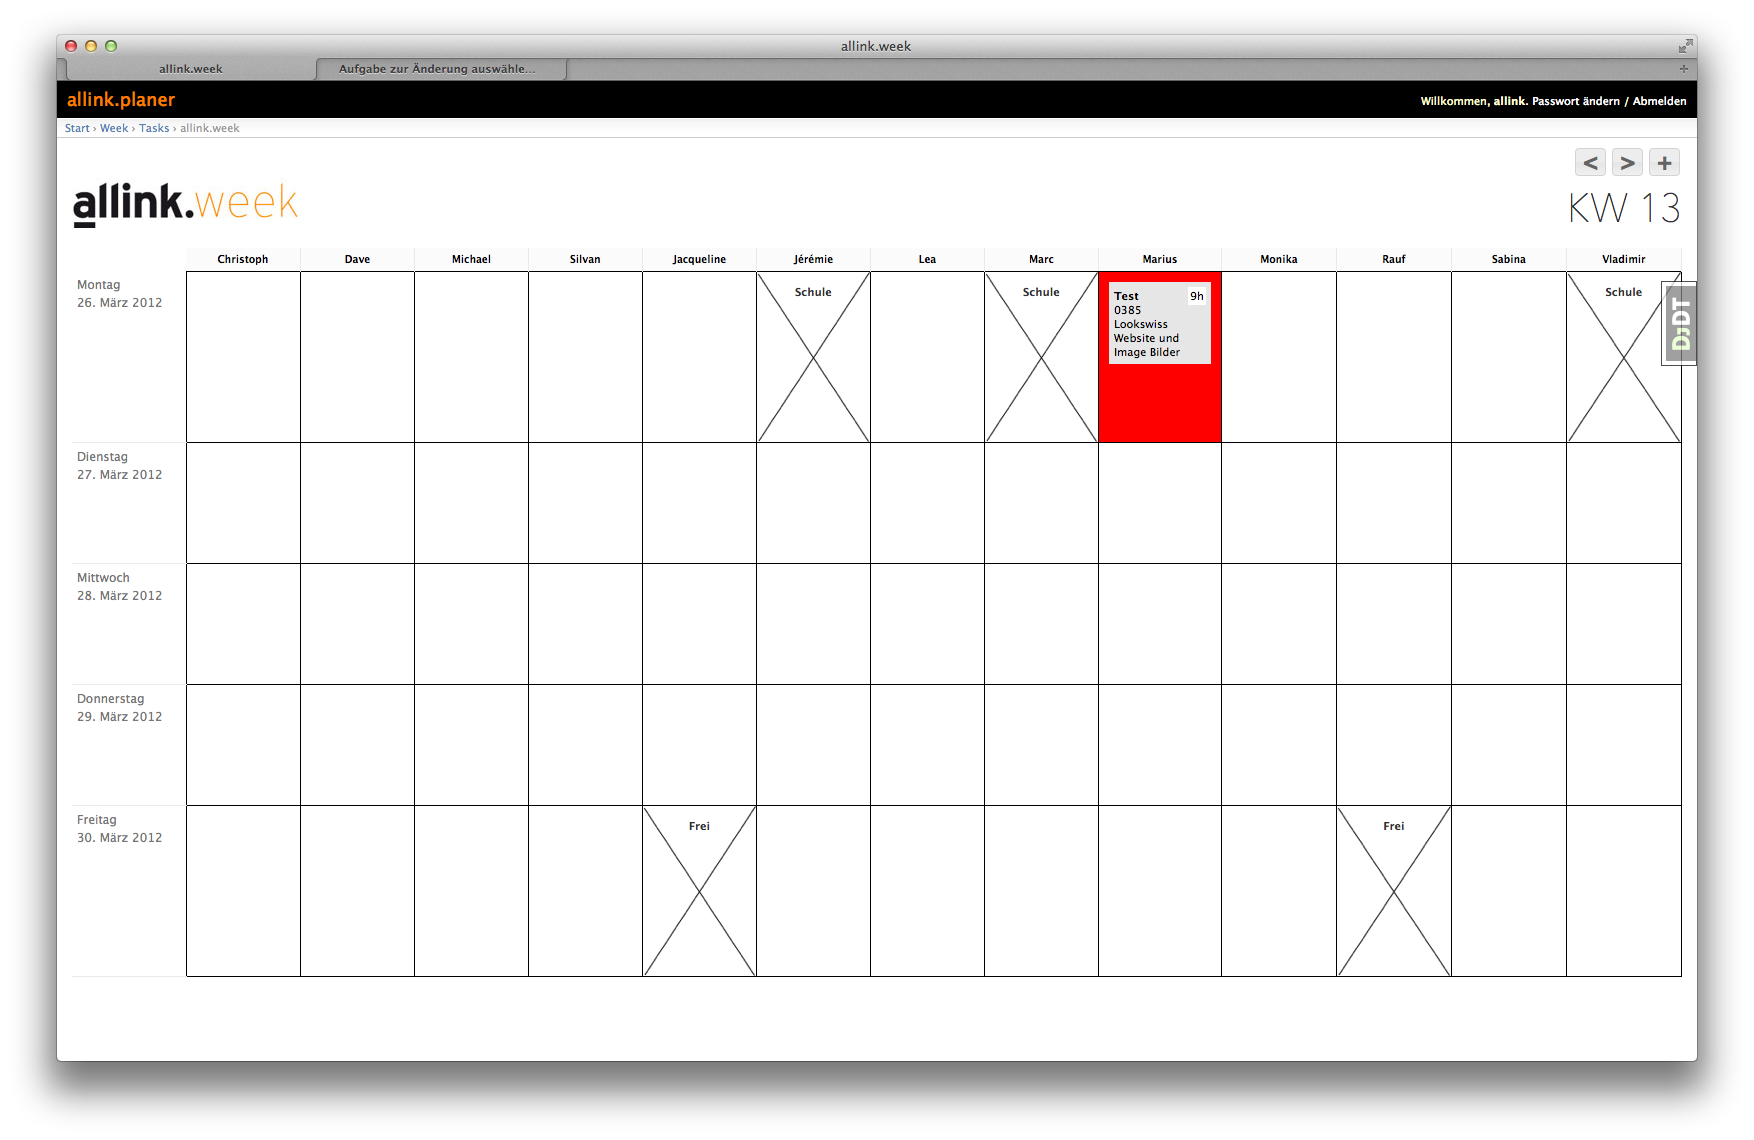
\includegraphics[height=0.85\textwidth,angle=90]{bilder/testing/warnmeldung.png}
    \caption{Abgedeckte Ziele: Nr. 17}
    \label{fig:bilder_testing_warnmeldung}
\end{figure}
\begin{figure}[htbp]
    \centering
        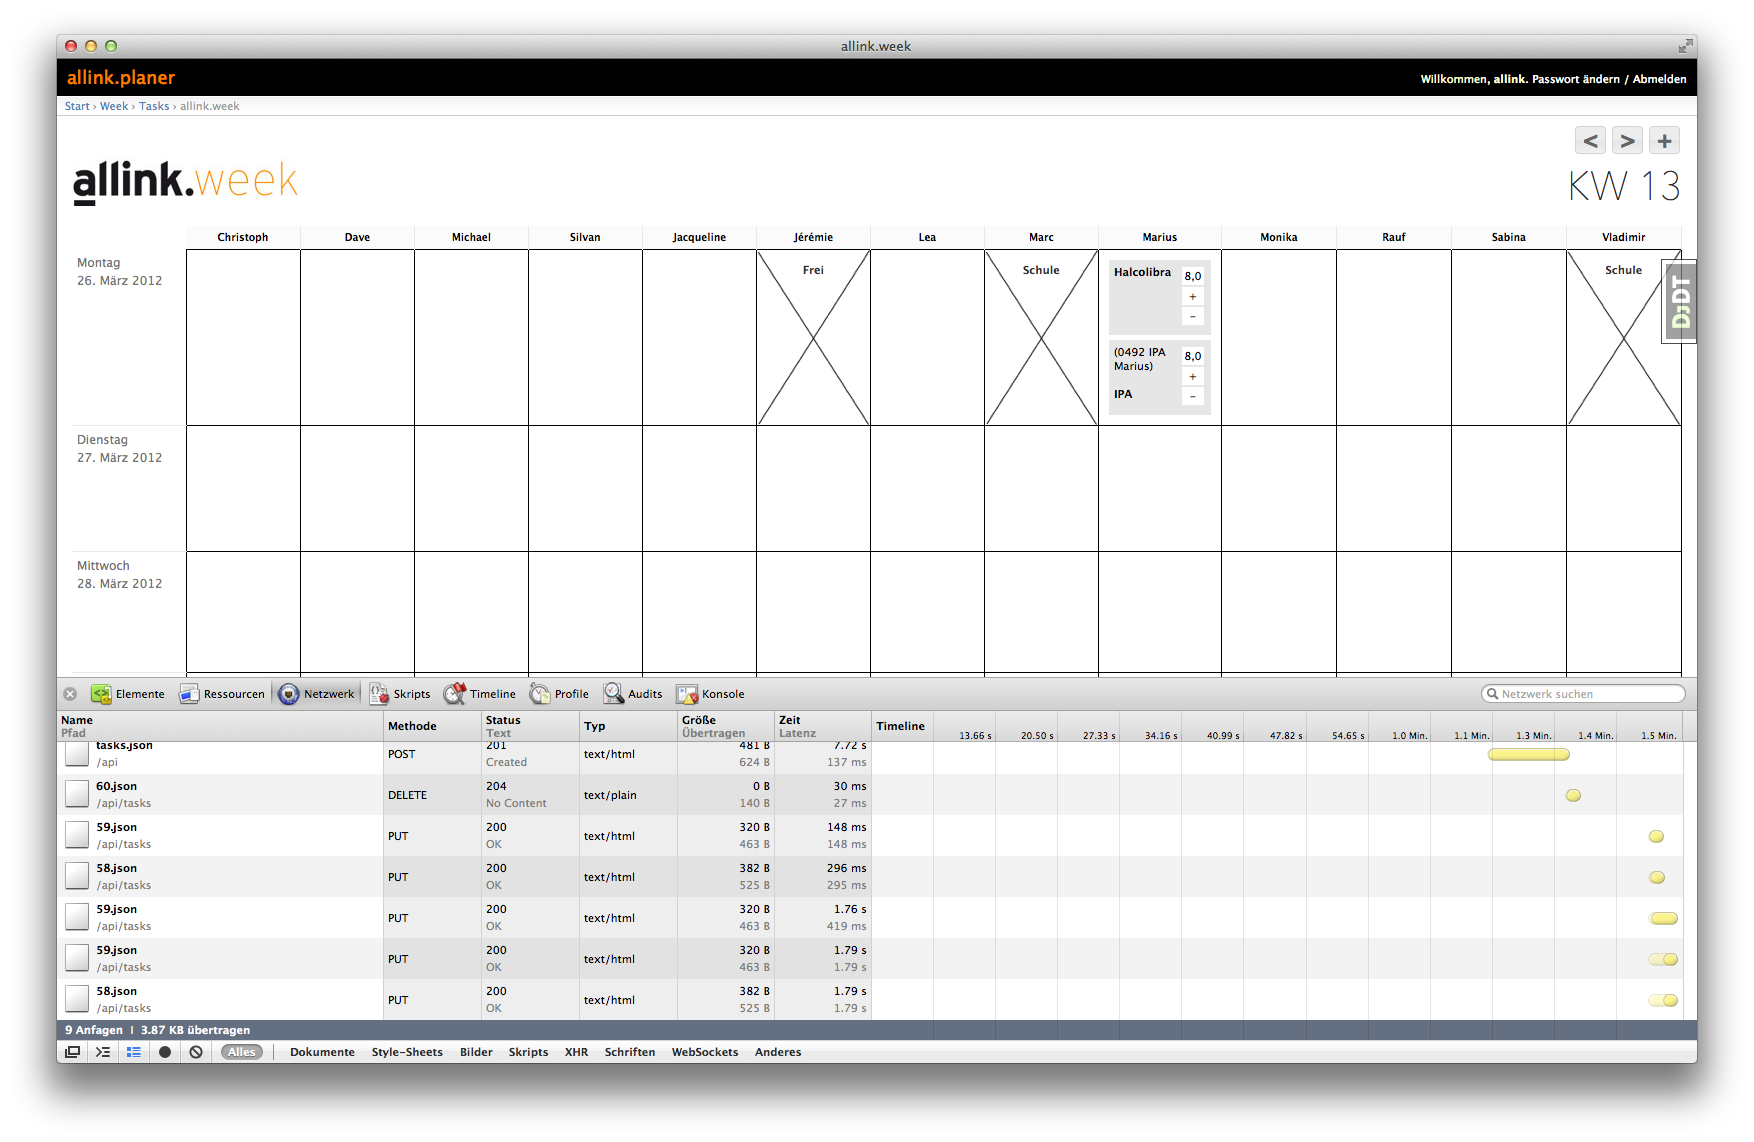
\includegraphics[height=0.85\textwidth,angle=90]{bilder/testing/tasks_sortieren.png}
    \caption{Abgedeckte Ziele: Nr. 18}
    \label{fig:bilder_testing_tasks_sortieren}
\end{figure}
\clearpage
\subsection{Resultate Testing}
Hier sind die Resulate der Tests aufgelistet:
\begin{table}[!ht]
\begin{center}
    \begin{tabular}{lll}
        \toprule Nr & MUSS-Funktion & erfüllt \\
        \midrule 1 & 1 & ja\\
        \midrule 2 & 2 & ja\\
        \midrule 3 & 3 & ja\\
        \midrule 4 & 4 & ja\\
        \midrule 5 & 5 & ja\\
        \midrule 6 & 6 & ja\\
        \midrule 7 & 7 & ja\\
        \midrule 8 & 8 & ja\\
        \midrule 9 & 9 & ja\\
        \midrule 10 & 10 & ja\\
        \midrule 11 & 11 & ja\\
        \midrule 12 & 12 & ja\\
        \midrule 13 & 13 & ja\\
        \midrule 14 & 14 & ja\\
        \midrule 15 & 15 & ja\\
        \midrule 16 & 16 & ja\\
        \midrule 17 & 17 & ja\\
        \midrule 18 & 18 & ja\\
        \bottomrule
    \end{tabular}
    \caption{Resultate Testfälle}
    \label{tab:testing_muss_funktionen_ziele}
\end{center}
\end{table}
\footnotetext{Eigene Darstellung}
\subsection{Field-Test}
Am 24.03. hat die Geschäftsführung an ihrer wöchentlichen Planungssitzung das Tool das erste Mal verwendet.
Dabei wurde das Tool auf seine Intuitivität geprüft. Am 26.03. habe ich Feedback erhalten um anfallende Anpassungen vornehmen zu können.
\subsection{Resultat Field-Test}
Das Tool wurde als gut befunden, die gewünschte Intuitivität ist umgesetzt worden und der Auftrag gilt seitens der Projektleitung als erfüllt.\\
Jedoch wurde die Bedienung, um ein Projekt auszuwählen, als zu umständlich empfunden. Es wird gewünscht, dass nach meiner IPA ein Formular mit ``autocompletion'' implementiert wird.